\subsection{Longitudinal flow fluctuations}

In nearly all traditional flow measurements the assumption is made that the 
  event-plane angles \psin\ do not change with $\eta$, i.e. that the \psin\
  are boost invariant.
This assumption is most clear in the event-plane and scalar-product methods
  of flow measurement,  where the \psin\ are measured at forward rapidities
  and the orientation of the reconstructed particles are then measured about
  these \psin~[HION-2016-06].
However multiple recent measurements at the LHC indicate the presence of 
  considerable longitudinal dynamics.
These include measurements from CMS of event-plane decorrelation in \ppb\ and \pbpb\ 
  collisions~\cite{CMS-HIN-14-012,CMS-HIN-15-008} and from ATLAS on flow-decorrelations~\cite{HION-2016-04}
  and forward-backward multiplicity fluctuations~\cite{HION-2015-13}.


In the ATLAS measurements in Ref.~\cite{HION-2016-04}, the flow decorrelation 
  is quantified by constructing a correlator $r_{n|n;1}$ defined as:
\begin{equation}
r_{n|n;1}(\eta)=%
  \frac{\langle \mathbf{v}_n(-\eta)\mathbf{v}_n^*(\eta_{\mathrm{ref}})\rangle}%
  {\langle \mathbf{v}_n(\eta)\mathbf{v}_n^*(\eta_{\mathrm{ref}})\rangle},
\end{equation}
where $\mathbf{q}_n$ is the normalized flow vector, and $\eta_{\mathrm{ref}}$ is 
  the reference pseudo-rapidity~\cite{HION-2016-04}.
The correlator,  $r_{n|n;1}$,  measures the relative difference between flow
  $v_ne^{in\psin}$ at $\eta$ and $-\eta$.
If flow were boost-invariant, then $r_{n|n;1}$ would equal unity.
However any  difference in the $\eta$ dependence of the flow magnitude
  $v_n$ and the event plane angle \psin\ will lead to $r_{n|n;1}$
  become smaller than unity.
The present ATLAS measurements of $r_{2|2;1}$ iover th 0--2.5 $\eta$ range 
  are shown in Figure~\ref{fig:atlas_r221} by the markers. 
It is observed that the $r_{2|2;1}$ is significantly smaller than unity 
  in central collisions, which indicates stronger flow decorrelation.
For a given centrality, $r_{2|2;1}$ decreases faster at low $\pT$ 
  that at higher-$\pT$.
In the 20--30\% mid-central $r_{2|2;1}$ decreases linearly with $\eta$, 
  however in the 0--5\% most central collisions there are indications
  that the decorrelations are possibly quadratic.

Repeating this measurement in Run~4 will lead to significant improvements 
  due to increased luminosity and especially due to increased tracking 
  acceptance in $\eta$ to $\pm4$ units.
Figure~\ref{fig:atlas_r221} also shows the ATLAS projections for 
  $r_{2|2;1}$ made for Run~4, indicated as dashed lines.
The ATLAS tracking acceptance in Run~4 will extend the $\eta$ range 
  to $\pm$4 units, but the projected measurement is made
  to $\pm$3.5 units, in order to leave a gap between the ITk and the 
  region of the forward calorimeter in which the reference measurement 
  is made ($4.4<|\eta|<4.9$).
The projections are made by fitting the existing data with a linear 
  function for the 20--30\% centrality case and with a quadratic 
  function for the 0--5\% centrality case.
It is seen that with the increased $\eta$ acceptance the non-linearlity 
  in the flow decorrelation can be studied in much more detail.


The longitudinal flow-decorrelation observables are sensitive to the 
  event by event fluctuations of the initial energy density profile 
  in the longitudinal direction. 
Thus precise measurement of these decorrelations should give
  a better understanding of the initial condition along the 
  longitudinal and in the development of full three-dimensional 
  viscous hydrodynamic models.
These would in turn result in a more accurate estimation of 
  $\eta/s$ from the model calculations.




\begin{figure*}[!htb]
\begin{center}
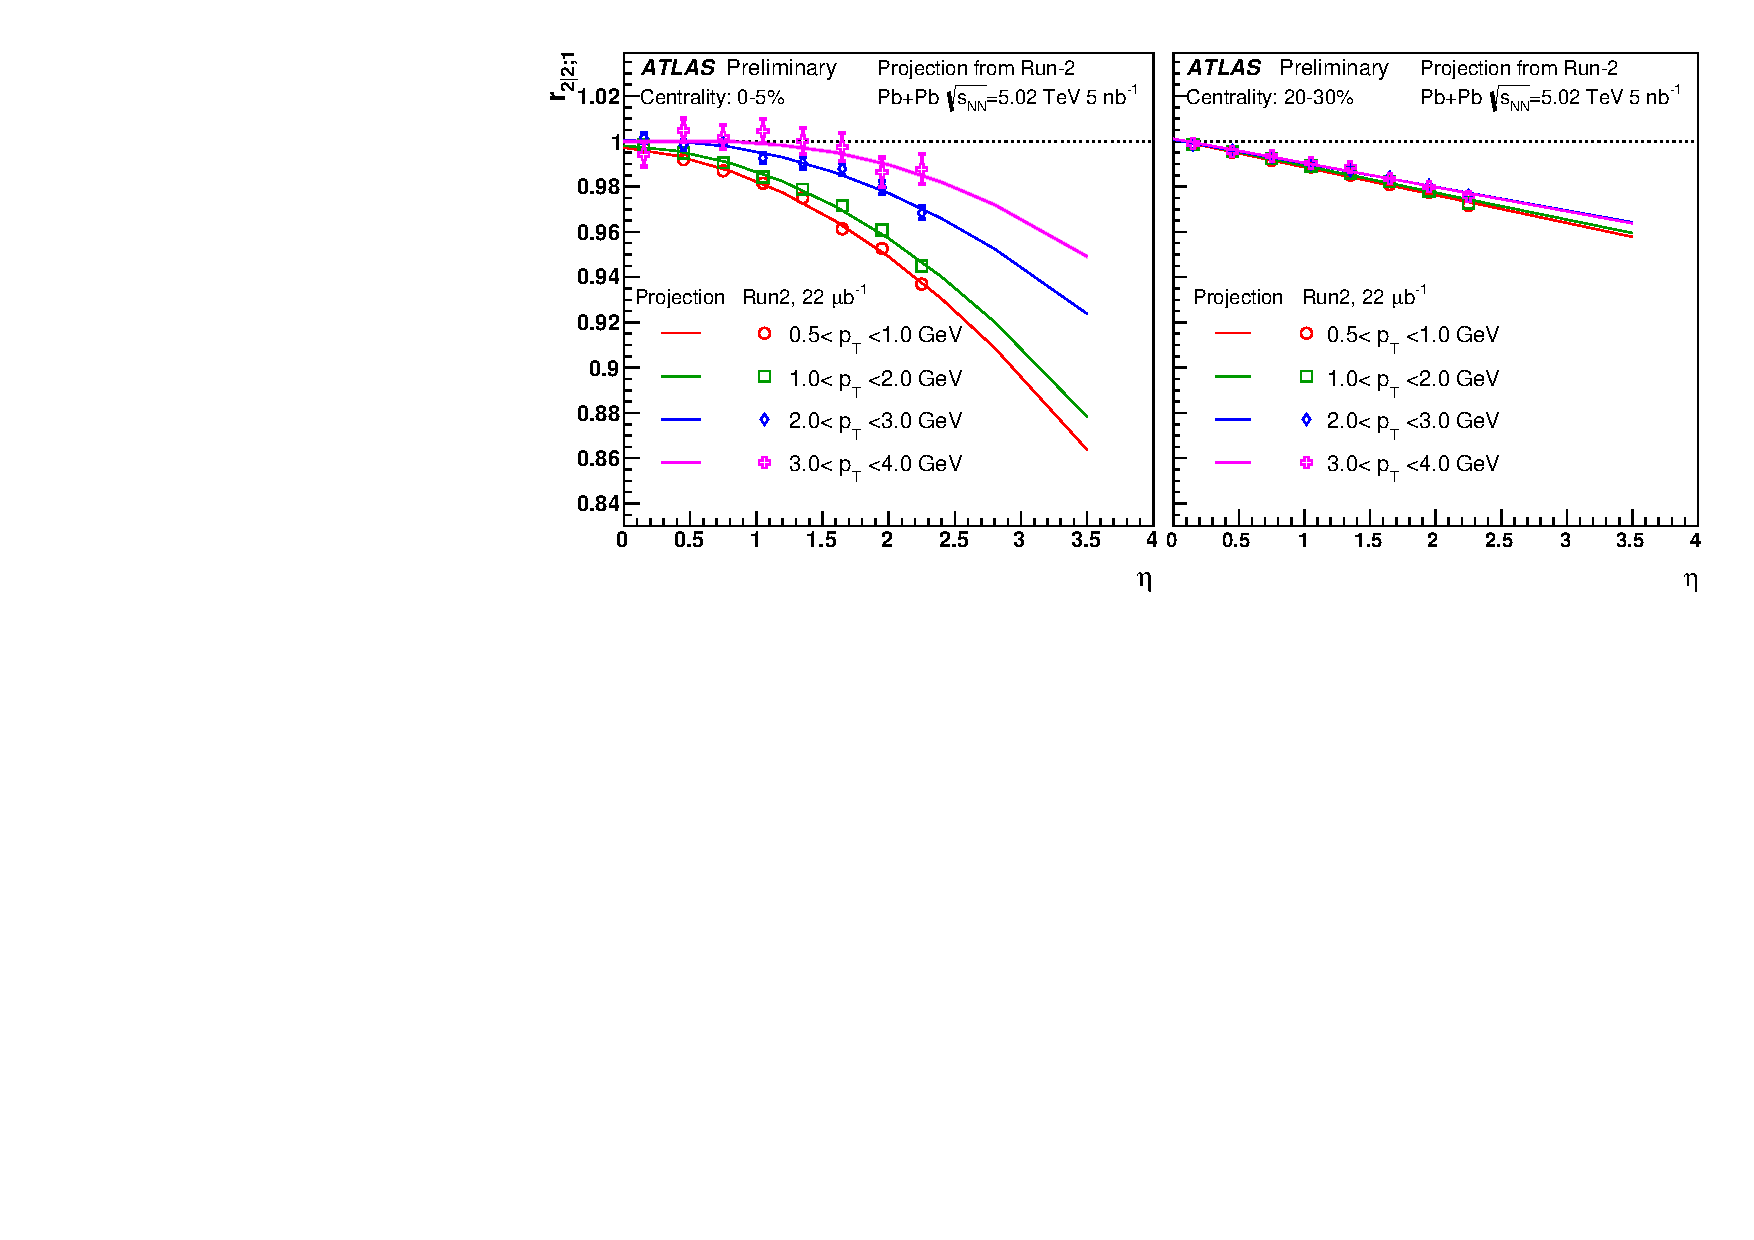
\includegraphics[width=0.8\textwidth]{\main/flow/figs/atlas_projection_r221}
\caption{
ATLAS measurements of the flow-decorrelation observable $r_{2|2;1}$ 
  as a function of $\eta$.
The markers indicate the present measurements from Ref.~\cite{HION-2016-04}.
The left and right panels show results for the 0--5\% and 20--30\%
  centrality intervals,  respectively.
The dashed lines show ATLAS projections of $r_{2|2;1}$ as expected to 
  be measured in Run~4.  
The width of the projection bands indicates the expected statistical uncertainty.
}
\label{fig:atlas_r221}
\end{center}
\end{figure*}

